
%
% Chapter 4
%

\chapter{FEEDBACK ANALYSIS}
\label{chap:strategyAnalysis}
Overall feedback strategies are stated in Chapter \ref{chap:strategy}, but not in detail. This chapter analyzes the strategies in more detail. For instance, this chapter covers the decision rules to use feedback or not, the selection of the best feedback strategy for our radio, and the design of the packet management system.

\section{Analysis of Feedback}
\label{secAnalysisFeedback}
In communication systems, especially in wireless communication systems, the received data can be corrupted by noise, channel fading and interference, which may result in data transmission errors. However, layers higher than the link layer usually are not prepared to deal with errors in the payload. To cope with the data transmission errors, fundamental retransmission schemes known as automatic repeat request (ARQ) and Hybrid ARQ (HARQ) have been designed \cite{ALarmoandMLindstromandMMeyerandGPelletierandJTorsnerandHWiemann2009}.

In the preliminary event, feedback was not implemented. Instead, linear transmission was used, which is described in the following procedure. A total of 15000 packets is transmitted. Packets are protected by a 32 bit cyclic redundancy check (CRC). If there is an error in a packet, the entire packet is dropped. After the transmission of the 15000 packets, the process repeats until 3 minutes pass. since packets that have been successfully received are retransmitted repeatedly, linear transmission has low efficiency. Since the arrangement of S1, D1, S2, and D2 in Figure~\ref{fig:CooperativeNodeAssignement} was used for the competitive match in the preliminary round, but the arrangement in Figure~\ref{fig:CompetitiveNodeGeometryFinalRound} was used for the competitive match in the final round, the feedback link in the final round had a higher SIR than that of the feedback link in the preliminary round. Consequently, feedback was used in the final competitive match.

In the cooperative match, the receiver in the source node would experience higher interference from the other source nodes. At first glance, the SIR is below 0 dB and feedback is not achievable in the cooperative match. However, if feedback is sent via the spectrum where there is no other signal and the source node implements a low pass filter, the SIR would be much higher than 0 dB and feedback becomes possible. Although feedback in the cooperative match is considered unreliable, feedback can still improve the efficiency of the radio when successfully received.

In this section, we will analyze the performance of different types of feedback and compare the results with the performance without feedback. The measurement metric is the total number of packets transmitted to complete the file transfer. For simplicity, we assume perfect synchronization and no loss of feedback packet during transmission.

\subsection{Stop and Wait ARQ}
\label{subsubStopAndWaitARQ}
In Stop and Wait ARQ, the source sends one packet at a time. After sending each packet, the source does not send any additional packets until it receives an acknowledgement (ACK) signal from the destination. After receiving a good packet, the destination sends an ACK. If the ACK does not reach the source before a certain time, known as the timeout, the source sends the same packet again \cite{AndrewTanenbaum2002}.

First, we consider a simplified Stop and Wait ARQ. Assume that packet transmission time, receiver data processing time and ACK time is 0. In other words, the source knows whether a packet has been transmitted successfully without delay and it can retransmit the packet until the packet is received without error. Let $N= 15000$ be the total number of packets (file size), $P_e$ be the packet error rate and $X_i$ be the number of transmissions for packet $i$ until it is successfully received. The probability of completing a packet $i$ in $k$ time transmissions  is
\begin{align}
\Pr \left( {X = k} \right) = {p_e}^{k - 1}\left( {1 - {p_e}} \right),\quad k = 1,2,3...
\end{align}
which is the geometric distribution.  If we assume that the $X_i$ ($i = 1, 2, ��, N$) are iid, the expected number of transmission for packet $i$ is
\begin{align}
E\left[ {{X_i}} \right] = \frac{1}{{1 - {p_e}}}.
\end{align}
The total expected number of packets transmitted to complete $N= 15000$ packets is the expected value of $M={\sum\limits_{i = 1}^N {{X_i}} }$, i.e.,
\begin{align}
E\left[ M \right] = E\left[ {\sum\limits_{i = 1}^N {{X_i}} } \right] = \frac{N}{{1 - {p_e}}}.
\end{align}

In the following analysis of other types of feedback, Matlab simulation will be used. To verify the simulation method, Stop and Wait ARQ is also simulated and calculation of the theoretical value is plotted as well.

In the simulation, we use BPSK modulation in a discrete-time Gaussian Interference Channel. No channel coding is used. The bit error rate can be expressed as
\begin{align}
{P_b} = Q\left( {\sqrt {\frac{{2{E_b}}}{{{N_0}}} } } \right) ,
\end{align}
where ${E_b}$ is the average bit energy, and the Q-function is the tail probability of the standard normal distribution, mathematically given as
\begin{align}
Q\left( x \right) = \frac{1}{{\sqrt {2\pi } }}\int_x^\infty  {\exp \left( { - \frac{{{u^2}}}{2}} \right)} du .
\end{align}
In the simulation, the ``rand'' function in Matlab is used to generate a uniformly distributed pseudorandom number on the open interval $\left( {0,1} \right)$ \cite{MatlabRand}. If the generated pseudorandom number is less or equal to $P_b$, the bit is considered to be in error, and if any bit in a packet is in error, the entire packet will be dropped. As a result
\begin{align}
{P_e} = 1 - {\left( {1 - {P_b}} \right)^l},
\end{align}
where $l$ is the number of bits in each packet.

\begin{figure}[tpb]
  \begin{center}
    \centerline{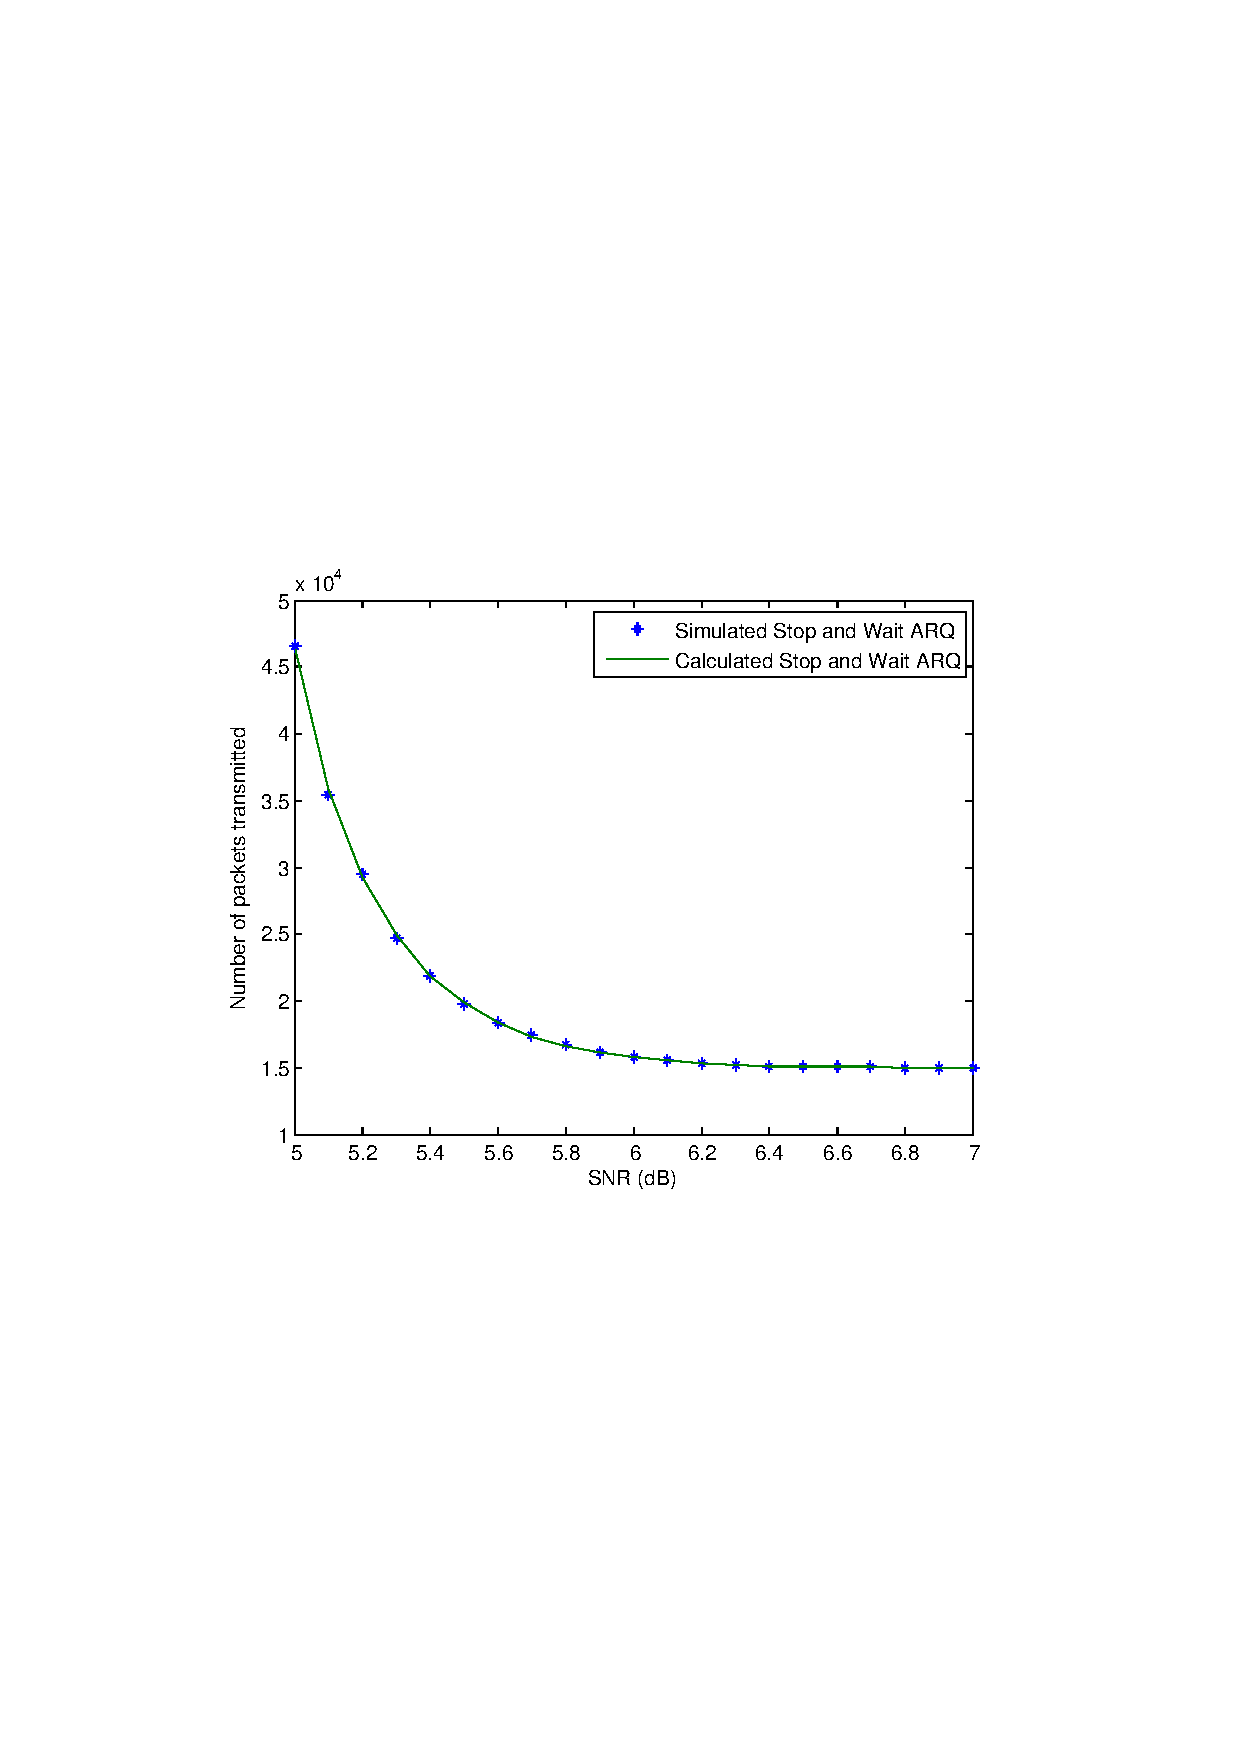
\includegraphics[width=140mm]{ComparisionSimulationVsCalculation.pdf}}
    \caption{Total number of packets transmitted to complete file transfer as a function of SNR. The simulated and theoretical results for Stop and Wait ARQ is shown for $N= 15000$ and $l=1440$.}
    \label{fig:ComparisionSimulationVsCalculation}
  \end{center}
\end{figure}

The simulation program counts the total number of packets transmitted to compete the file. For simplicity, a packet size of $l=1440$ bits is used. The simulation program is run 100 times, and the simulation results are averaged to reduce the mean squared estimation error. Figure~\ref{fig:ComparisionSimulationVsCalculation} illustrates total number of packets transmitted to complete file transfer using stop and wait ARQ, companying simulation to calculation. It shows that the simulation result closely matches the theoretical result, and the simulation method can be used in the following feedback analysis. From the figure, as SNR increases, the total number of packets transmitted decreases until approaching the lower bound, the file size 15000 packets.



\subsection{Transmission without Feedback}
\label{subsubNofeedback}
In the situation without feedback, linear transmission is used, that is, 15000 packets are transmitted from the beginning to the end periodically until 3 minutes pass. The transmission of 15000 packets from the beginning to the end is defined as one round.

Let $M_i$ be the round number when packet $i$ is successfully received, where $i=1, 2, 3 ...$. In rounds 1 to $M_i-1$, packet $i$ is in error. We assume $M_i$ is independent with $M_j$ for $i\neq j$.Then
\begin{align}
\Pr \left( {{M_i} \le m} \right) = 1 - {P_e}^m.
\end{align}

Let $M$ be the round number when all packets are finally successfully received. We have
\begin{align}
M=\mathop {\max }\limits_{i \in \left\{ {1,2,...,N} \right\}} \left\{ {{M_i}} \right\}.
\end{align}
The total number of packets transmitted to complete file transfer is on the interval $\left( {\left( {M - 1} \right)N,MN} \right]$. For simplicity, The upper bound $MN$ is used in comparison. Then for $ m=1,2,3...$
\begin{align}%{rcl}
%\begin{split}
\Pr \left( {M \le m} \right) &= \Pr \left( {\mathop {\max }\limits_{i \in \left\{ {1,2,...,N} \right\}} \left\{ {{M_i}} \right\} \le m} \right)&\\
 &= \Pr \left( {{M_1} \le m,{M_2} \le m,...,{M_N} \le m} \right)&\\
 &= {\left( {1 - {P_e}^m} \right)^N},&
\label{PMcdf}
\end{align}
and we can obtain the probability mass function
\begin{align}
\Pr \left( {M = m} \right) &= \Pr \left( {M \le m} \right) - \Pr \left( {M \le m - 1} \right)&\\
                           &= {\left( {1 - {P_e}^m} \right)^N} - {\left( {1 - {P_e}^{m - 1}} \right)^N},\quad m = 1,2,3....&
\end{align}
The expectation of $M$ is
\begin{align}
%\begin{split}
E\left[ M \right] &= \sum\limits_{m = 1}^\infty  {m\Pr \left( {M = m} \right)}&\\
\label{ExpectionM} \nonumber
&= \sum\limits_{m = 1}^\infty  {m\left[ {{{\left( {1 - {P_e}^m} \right)}^N} - {{\left( {1 - {P_e}^{m - 1}} \right)}^N}} \right]  }&\\
&= \sum\limits_{m = 1}^\infty  {m\left[ {\sum\limits_{k = 0}^N {{{\left( { - 1} \right)}^k} {N \choose k} } {P_e}^{mk} - \sum\limits_{k = 0}^N {{{\left( { - 1} \right)}^k}{N \choose k}} {P_e}^{\left( {m - 1} \right)k}} \right]}.&
%\end{split}
\end{align}
When $k=0$, ${\sum\limits_{k = 0}^N {{{\left( { - 1} \right)}^k}{N \choose k}} {P_e}^{mk} - \sum\limits_{k = 0}^N {{{\left( { - 1} \right)}^k}{N \choose k}} {P_e}^{\left( {m - 1} \right)k}}=0$. We have
\begin{align}
E\left[ M \right] &= \sum\limits_{k = 0}^N {{{\left( { - 1} \right)}^k}{N \choose k}} \sum\limits_{m = 1}^\infty  {m\left[ {{P_e}^{mk} - {P_e}^{\left( {m - 1} \right)k}} \right]}&\\ \nonumber
&= \sum\limits_{k = 1}^N {{{\left( { - 1} \right)}^k}{N \choose k}} \frac{{\left( {{P_e}^k - 1} \right)}}{{{P_e}^k}}\sum\limits_{m = 1}^\infty  {m{P_e}^{mk}}&\\ \nonumber
&= \sum\limits_{k = 1}^N {{{\left( { - 1} \right)}^k}{N \choose k}} \frac{{\left( {{P_e}^k - 1} \right)}}{{{P_e}^k}}\frac{{{P_e}^k}}{{{{\left( {1 - {P_e}^k} \right)}^2}}}&\\
&= \sum\limits_{k = 1}^N {{{\left( { - 1} \right)}^{k + 1}}{N \choose k}} \frac{1}{{1 - {P_e}^k}}.&
\label{ExpectationEMNoFeedback}
\end{align}

\begin{figure}[tpb]
  \begin{center}
    \centerline{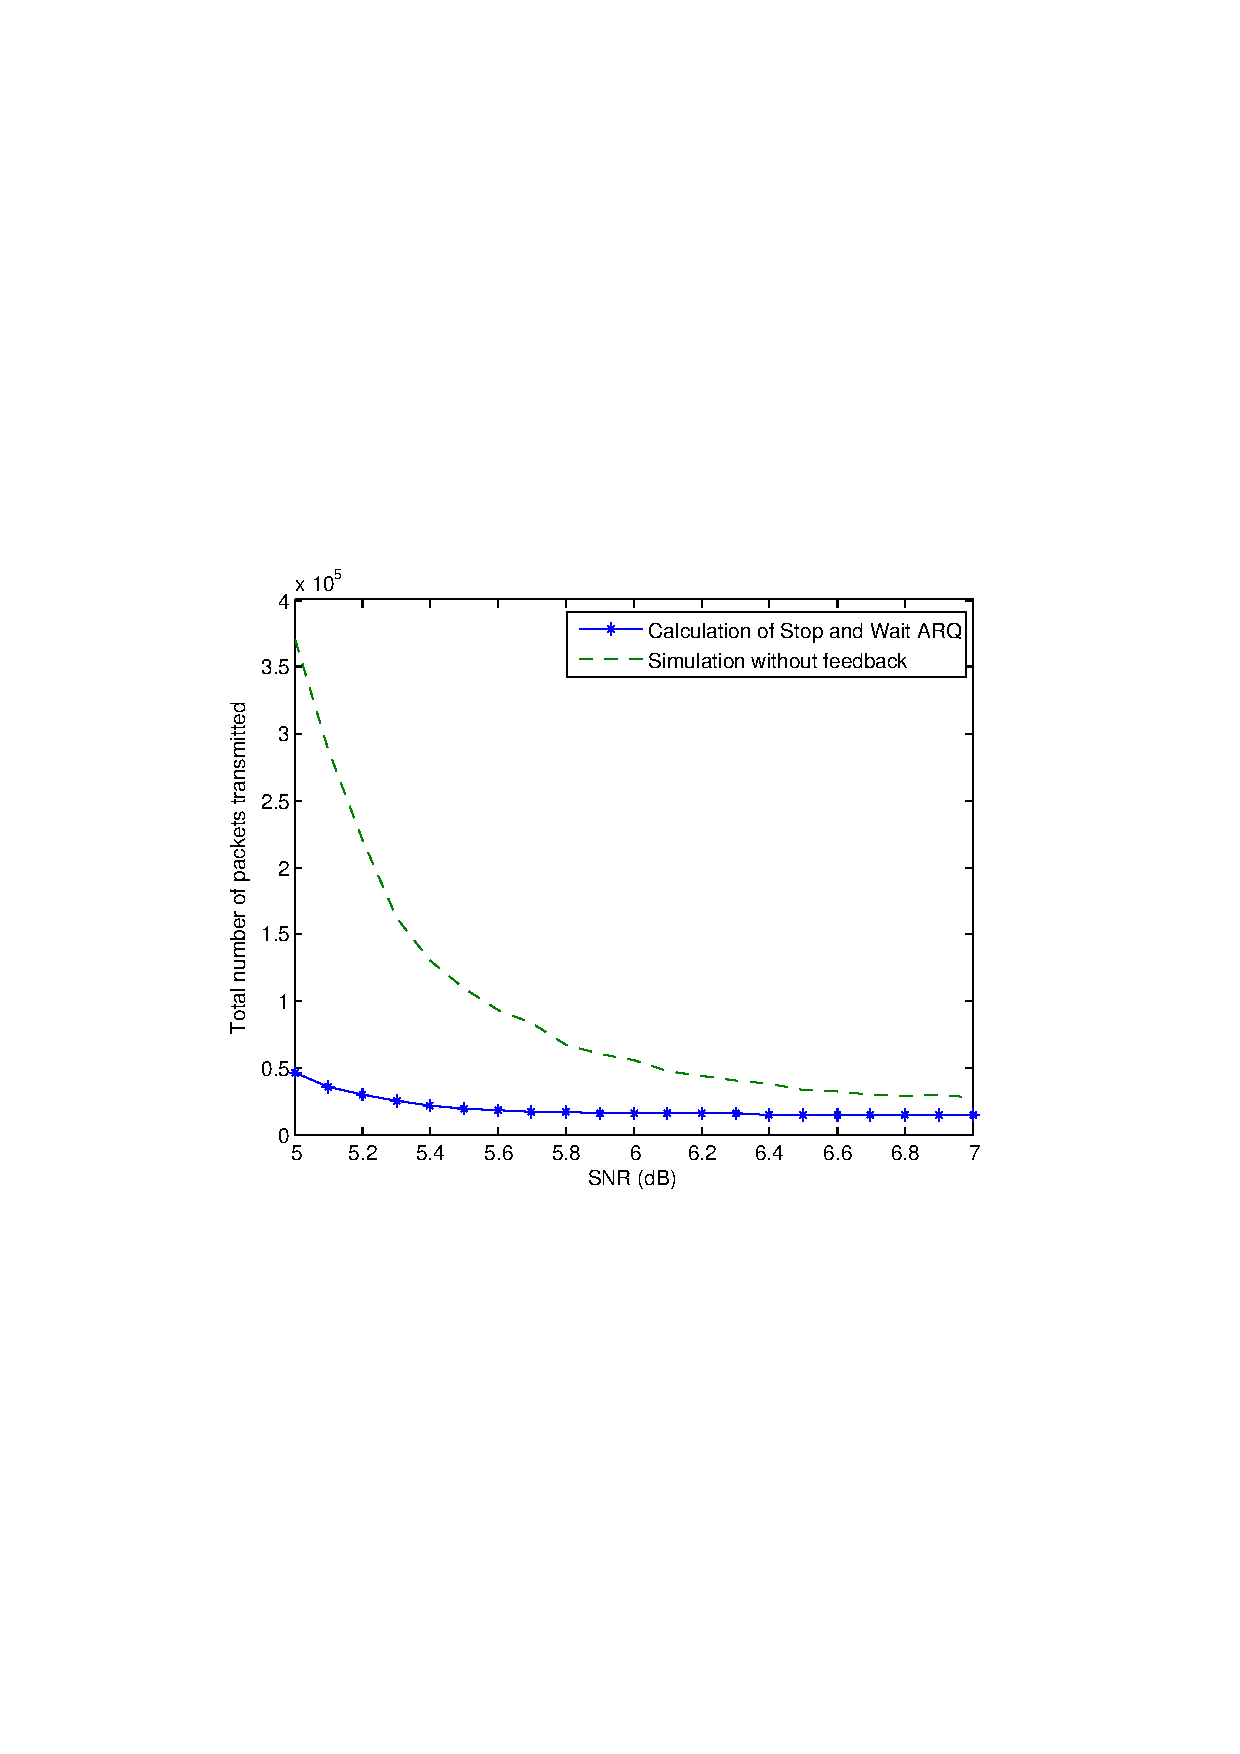
\includegraphics[width=140mm]{NoFeedbackSimulatoinandARQ.pdf}}
    \caption{Total number of packets transmitted to complete file transfer as a function of SNR for Stop and Wait ARQ  compared against that for Linear Transmission.}
    \label{fig:WithAndWithoutFeedback}
  \end{center}
\end{figure}

The precision of Matlab is not high enough to calculate $1 - {P_e}^k$, and a numeric value cannot be derived from (\ref{ExpectationEMNoFeedback}). Therefore simulation is primarily used to compare the performance of Stop and Wait ARQ and that  of Linear Transmission without feedback.

Figure~\ref{fig:WithAndWithoutFeedback} shows the simulation result with and without Stop and Wait ARQ. Without feedback, the total number of transmitted packets increases dramatically. As ${\rm{SNR}} \to \infty$, ${P_e} \to 0$, and from (\ref{ExpectionM}), we can conclude
\begin{align}
\mathop {\lim }\limits_{{\rm{SNR}} \to \infty } E\left[ M \right] = \mathop {\lim }\limits_{{\rm{SNR}} \to \infty } \sum\limits_{m = 1}^\infty  {m\left[ {{{\left( {1 - {P_e}^m} \right)}^N} - {{\left( {1 - {P_e}^{m - 1}} \right)}^N}} \right]}  = 1.
\end{align}
As a result, the total number of transmitted packets converges to 15000 as ${\rm{SNR}} \to \infty$.



\subsection{Highest Consecutive Packet Number Feedback}
In both the competitive and the cooperative matches, sending less feedback data allows for more time to be used in forward link data transmission. In Stop and Wait ARQ, every packet is acknowledged, which may require a significant amount of feedback data. Another feedback scheme, called Highest Consecutive Packet Number Feedback will be explored to reduce the amount of feedback data. In Highest Consecutive Packet Number Feedback, only one number is sent in the feedback data to indicate that all packets with packet number less than or equal to the number have been successfully received. Once the source receives the highest consecutive packet number, the next round of transmission starts with the highest consecutive packet number plus one.

\begin{figure}[tpb]
  \begin{center}
    \centerline{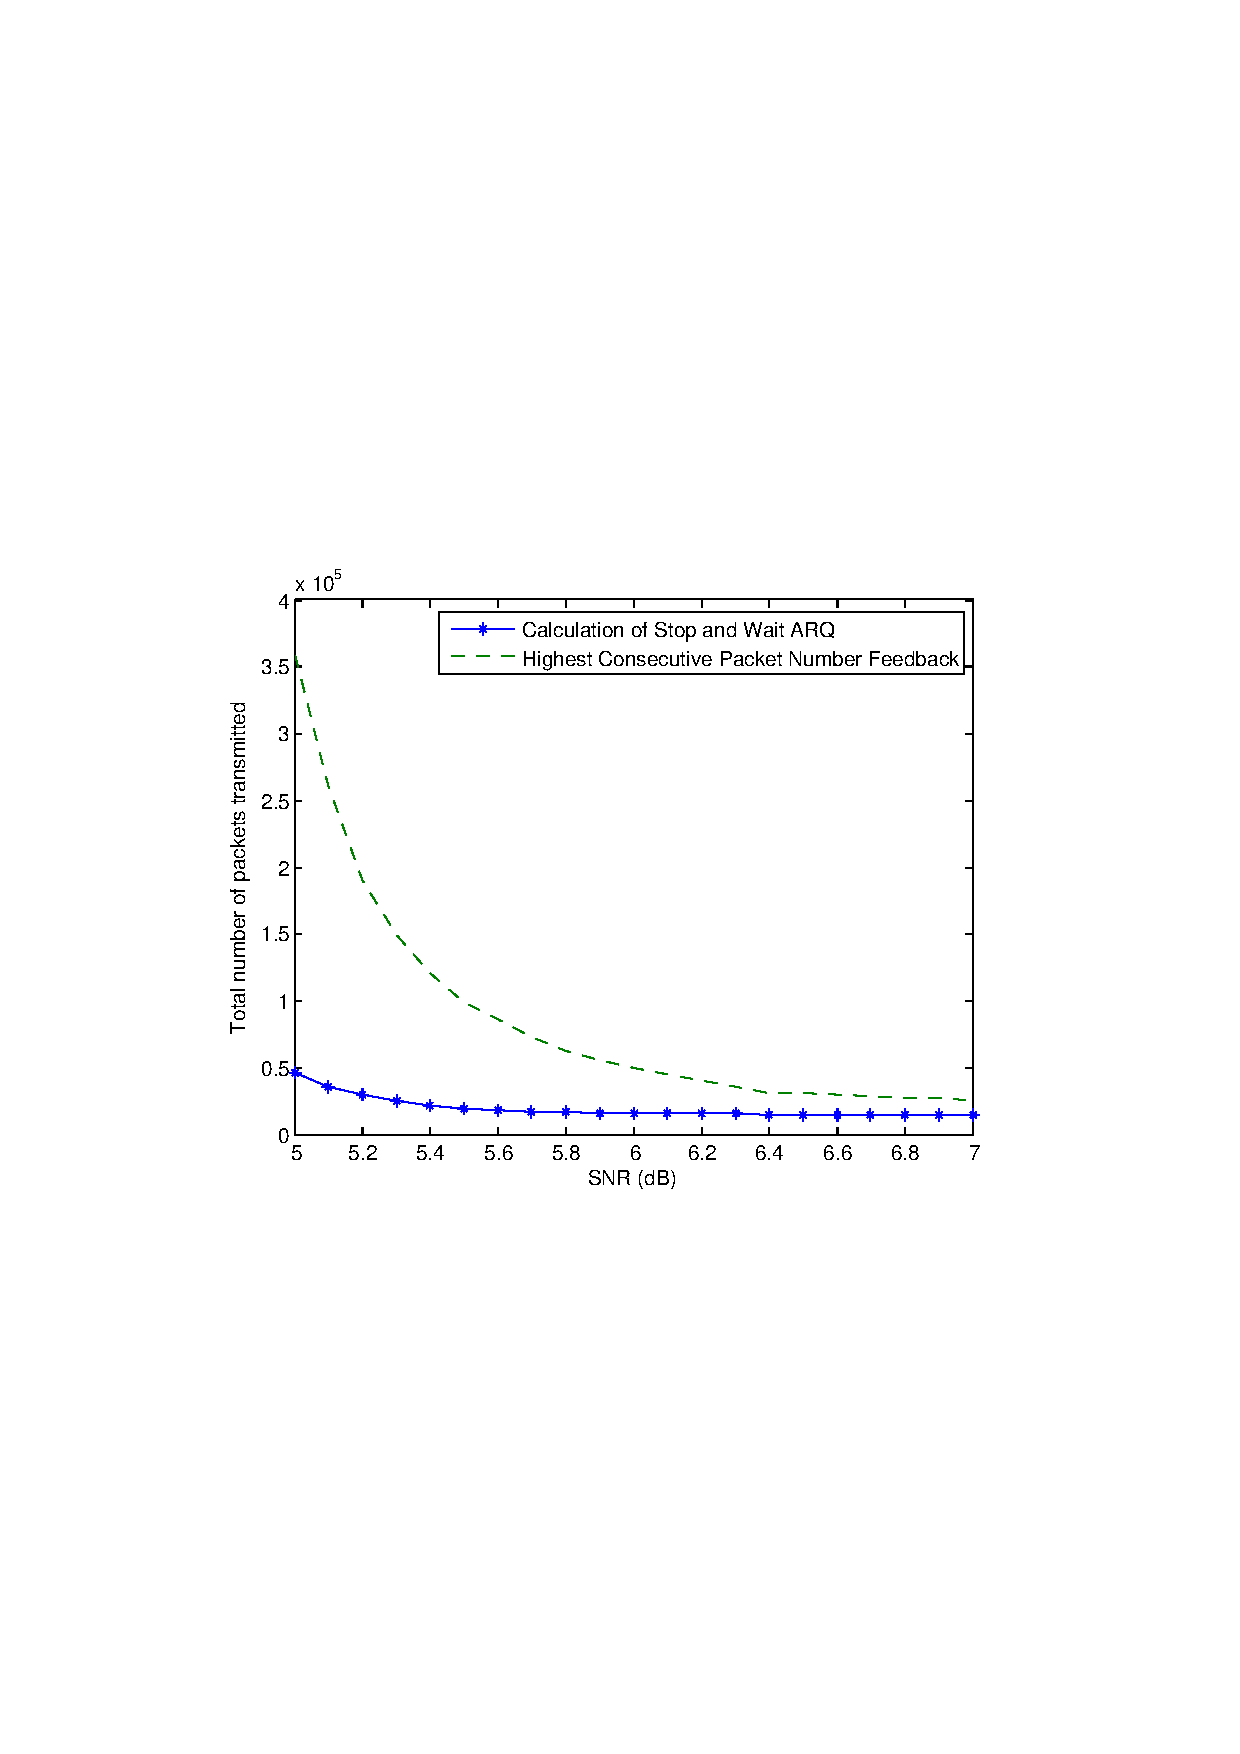
\includegraphics[width=140mm]{HighestPktNoFeedbackSimulatoinandARQ.pdf}}
    \caption{Total number of packets transmitted to complete file transfer for Stop and Wait ARQ compared against that for Highest Consecutive Packet Number Feedback.}
    \label{fig:HighestPktNoFeedbackSimulatoinandARQ}
  \end{center}
\end{figure}

Figure~\ref{fig:HighestPktNoFeedbackSimulatoinandARQ} illustrates the total number of packets transmitted to complete file transfer for Stop and Wait ARQ  and for Highest Consecutive Packet Number Feedback. The total number of transmit packets is much higher than that of Stop and Wait ARQ. By compare Figure~\ref{fig:WithAndWithoutFeedback} with Figure~\ref{fig:HighestPktNoFeedbackSimulatoinandARQ}, we see that the total number of packets transmitted is only slightly lower in Highest Consecutive Packet Number Feedback than in Linear Transmission.

Highest Consecutive Packet Number Feedback greatly reduces the amount of feedback data, but has low efficiency.


\subsection{Group Feedback}
Stop and Wait ARQ and Highest Consecutive Packet Number Feedback are two extreme situations in terms of performance and cost. Another type of feedback, Group Feedback, is explored to balance the performance and cost. In Group Feedback, one feedback number acknowledges that a group of packets with a given consecutive packet number has been received. The default method is to transmit all the unacknowledged file packets from the lowest to the highest packet number round by round. Let the group size be $S$. A group feedback number $k$ means packets with packet number $(S-1)k+1$ to $Sk$ have been received.

For example, if $S=5$ and the source receives a feedback number $k=1$, it means the receiver has successfully received packets with number 1 to 5. If $S=1$, Group Feedback is equivalent to Stop and Wait ARQ. Within each group, say Group $i$, it is equivalent to transmission without feedback with $N=S$ as discussed in Section \ref{subsubNofeedback}. If $S=15000$, the total packet number in the file, Group Feedback is equivalent to transmission without feedback. From (\ref{ExpectationEMNoFeedback}), the expected total number of packets transmitted to complete file transfer
\begin{align}
E\left[ {{n_t}} \right] = N\sum\limits_{k = 1}^S {{{\left( { - 1} \right)}^{k + 1}}{S \choose k}} \frac{1}{{1 - {P_e}^k}},
\end{align}
which is not good for numeric calculation in Matlab because the precision of Matlab is not high enough as the discussed in Section \ref{subsubNofeedback}. We again use simulation to compare performance.

Another concept, called feedback compression rate (denoted $R_f$) is used. Suppose, one feedback packet can represent $n_f$ data packets when $S=1$. Feedback compression rate can be defined as
\begin{align}
{{\rm{R}}_f} = \frac{{{n_f}}}{S}.
\end{align}
Typical value of $n_f$ ranges from 1/30 to 1/12 in our radios. Consider a worse situation, and $n_f=0.2$ is used. Suppose the number of packets in the data link to be $n_d$. The total number of packets in both the data link and the feedback link can be expressed as
\begin{align}
{n_t} = {n_d}\left( {1 + {{\rm{R}}_f}} \right) = {n_d}\left( {1 + \frac{{{n_f}}}{S}} \right).
\end{align}

Figure~\ref{fig:GroupFeedback} illustrates the simulation result of group feedback. In low SNR, such as 5 dB, the total number of total transmitted packets in both links increases dramatically, as the group size $S$ increases. It shows $S=1$ is better in low SNR. In relatively high SNR, such as 7 dB, group feedback with $S>1$ is slightly better than that with $S=1$. In both the competitive and cooperative matches, harsh environments with low SNR, should be considered. Therefore, $S=1$, namely Stop and Wait ARQ, is preferred.

\begin{figure}[tpb]
  \begin{center}
    \centerline{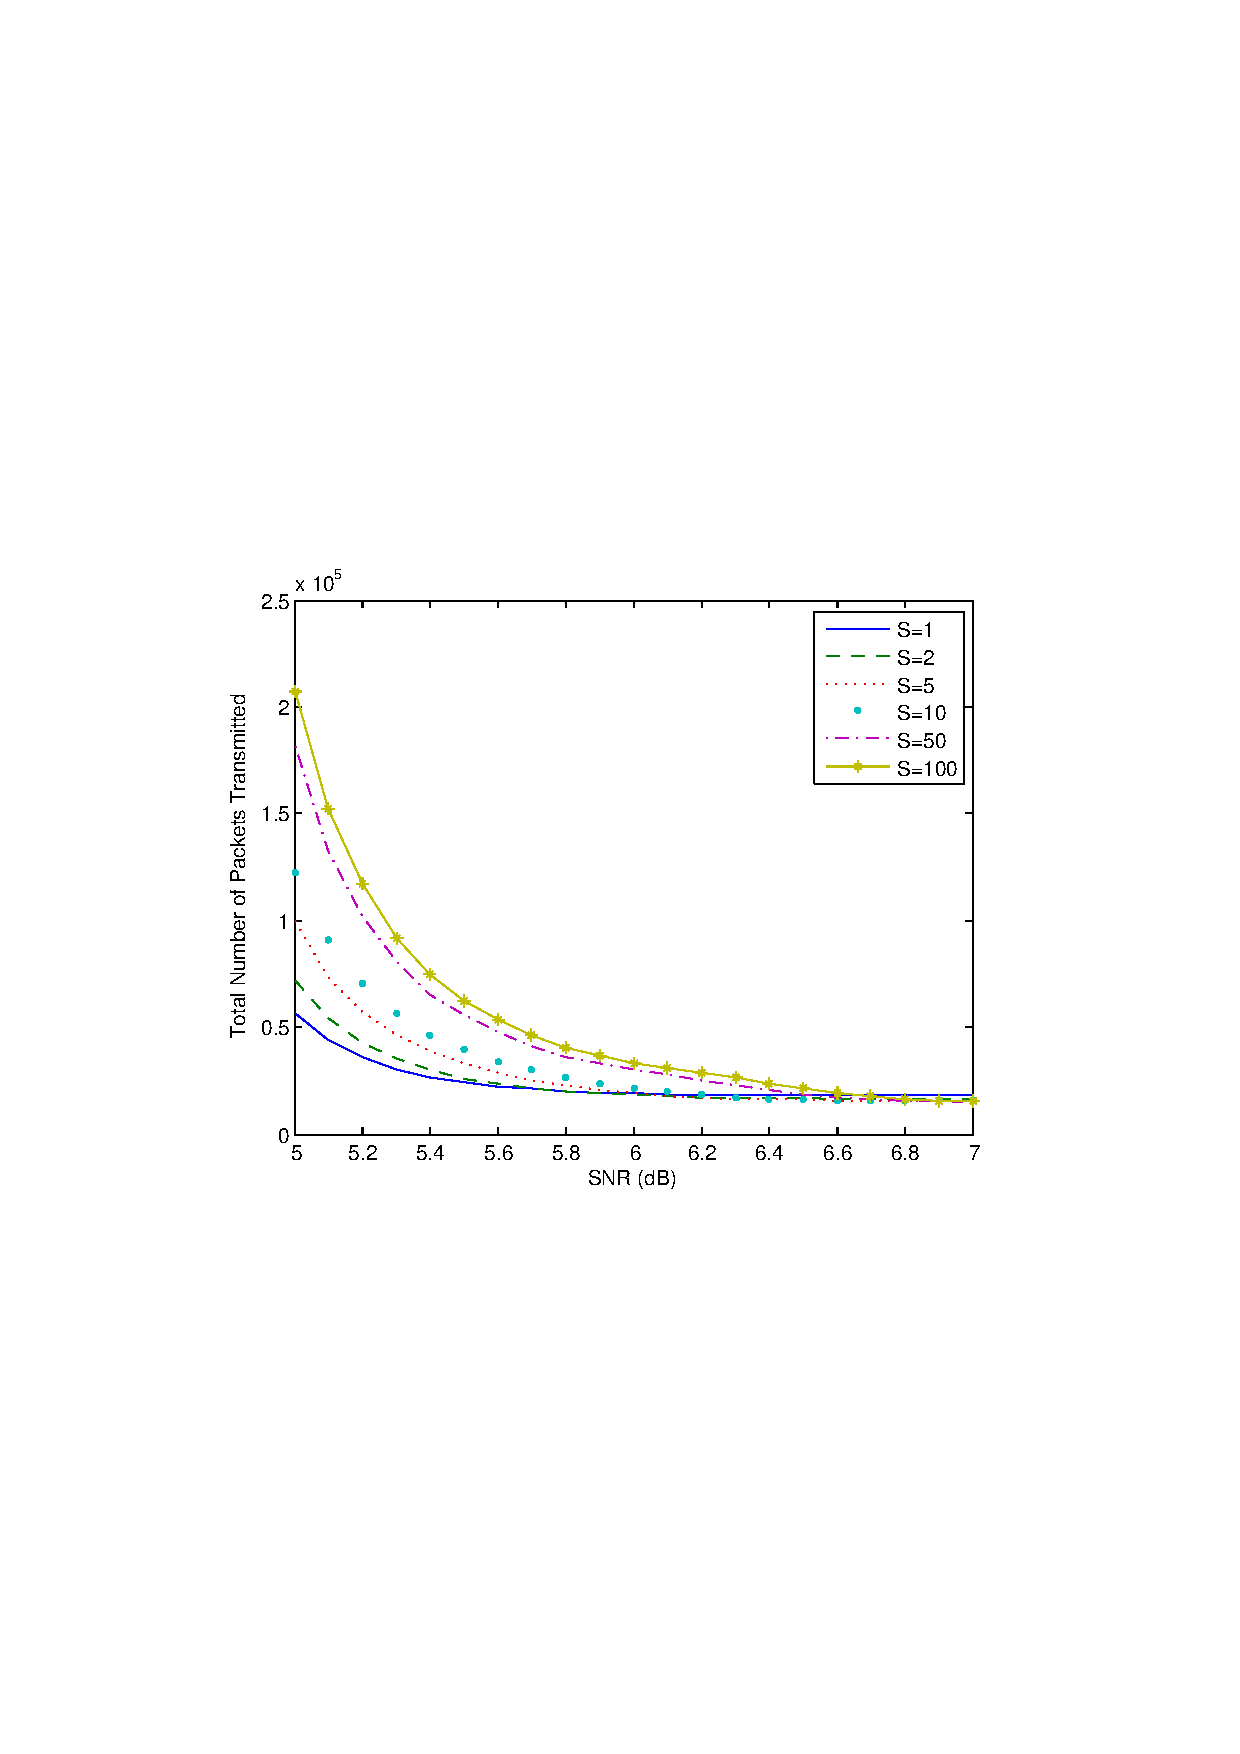
\includegraphics[width=140mm]{GroupFeedback.pdf}}
    \caption{Total number of packets transmitted in both data link and feedback link to complete file transfer for Group Feedback. $n_f=0.2$.}
    \label{fig:GroupFeedback}
  \end{center}
\end{figure}

It seems that group feedback is useless in our radio, but a modified version of group feedback can be used to significantly improve the feedback performance when practical situations are considered, which will be discussed in Section \ref{feedbackDesign}.

\subsection{Sliding Window ARQ}
In the Stop and Wait ARQ discussed in Section \ref{subsubStopAndWaitARQ}, the feedback delay, including data transmission time, receiver data processing time and ACK time, is assumed to be 0, but the assumption does not apply in practice. Sliding Window ARQ is used to solve the problem of feedback delay in the manner described below.

In Sliding Window ARQ, the source maintains a window of source packets. Suppose the size of the window is $S_w$, which corresponds to shift registers of size $S_w$ containing the packets to be transmitted. The registers are assigned a serial number as $\left( {{\rm{1, 2, }}...{\rm{, }}{{\rm{S}}_w}} \right)$. The source transmits the packet in the first register and then the second packet even if it has not received an ACK of the first packet from the destination. If the source transmits all the $S_w$ packets in the transmitting window, it will repeat the process by transmitting the packet in the first register and so on. Once the source obtains an ACK of any packet in the shift registers, the shift registers shift to flush that packet and get a new packet and put it in register $S_w$.

The key parameter in Sliding Window ARQ is the window size $S_w$. The window size should be large enough to ensure that the time of one transmission round of data in the window is larger than the feedback delay. If the window size condition is satisfied, the performance of Sliding Window ARQ is equal to that of Stop and Wait ARQ.


\section{Feedback Design}
\label{feedbackDesign}
Based on the analysis in Section \ref{secAnalysisFeedback}, Sliding Window ARQ will be used in our radio. However, the analysis of feedback is based on the assumption that the reverse link (feedback link) is reliable. Actually, in both competitive and cooperative match, the reverse link cannot guarantee 100 $\%$ reliable transmission, even with channel coding, because of the unpredictable interference from the competitor and cooperators. There is a certain non-zero probability that acknowledgements from the receiver may be lost or corrupted.

To compensate for the unreliability of the reverse link, the destination keeps sending acknowledgements of all the received packets round by round. However, another problem arises. If every single packet is acknowledged by a feedback number, the total feedback data would increase dramatically as the number of successfully received packet increases. We will use a complex feedback that combines the Sliding Window ARQ, Highest Consecutive Packet Number Feedback, and Group Feedback. For this complex feedback,  there is a number indicating the highest consecutive packet number in every feedback packet, and the rest of the acknowledgements are represented by Group Feedback with multiple group size. The values $S =5$, $S=20$, $S=100$ and $S=500$ are used for cooperative radio and $S =5$, $S=30$ and $S=200$ are used for competitive radio. If all packets in a larger group have been received, a single feedback number will be sent to acknowledge all packets in the group have been received. Otherwise, a smaller group will be used and so on.

\subsection{Bit level design for cooperative radio}

In cooperative radio, each physical-layer packet has 116 bytes to carry data and 4 bytes for CRC check. Five bytes are used for a header, and 111 bytes are used to carry a sub-packet. As a result, each application packet of size 1440 bytes from the server is divided into 13 sub-packets. The first 12 sub-packets have 111 bytes and the last one has 108 bytes. In the header, two bytes are used for indicating the packet number and one byte is used for the sub-packet number. The left two bytes in the header are reserved.

In the feedback link, a physical-layer packet also has 116 bytes of data. One byte is used to indicate whether all the packets have been successfully received, and two bytes are used for Highest Consecutive Packet Number Feedback. For all the remaining bytes, 4 bytes are used as a group. The first two bytes indicate the packet number and 13 bits of the other two bytes are used as bitmap to show whether each individual sub-packet has been received. If group feedback is used, hexadecimal numbers 3FFF, 7FFF, BFFF and FFFF are set in the two-byte bitmap to stand for group feedback with group size $S =5$, $S=20$, $S=100$, and $S=500$ respectively.


\subsection{Bit level design for competitive radio}
In competitive radio, uncoded QPSK with rate 1, QPSK with rate 1/2 repetition code, BPSK with 1/2 repetition code and BPSK with 1/4 repetition code lead to MAC payload sizes of 236 bytes, 116 bytes, 56 bytes and 26 bytes respectively. To meet the requirement of variable MAC payload size, a sub-packet size of 23 bytes is used. Three bytes are added to the sub-packet to indicate the packet number and sub-packet number. Therefore each sub-packet needs 26 bytes in total.  Each 1440-byte application packet is divided into 63 sub-packets.  The first 62 sub-packets each has 23 bytes, and the last one has 14 bytes. Each MAC payload tries to fill as many sub-packets as possible.

In the feedback, QPSK with rate 1/2 repetition code is used and each MAC payload has 116 bytes. As in the cooperative radio, one byte is used to indicate whether all the packets have been successfully received, and two bytes are used for Highest Consecutive Packet Number Feedback. If not all the sub-packets in a packet are received, the feedback data has 10 bytes. Two of bytes are used for the packet number, and the other 8 bytes form a 64-bit bitmap to indicate whether each sub-packet is received. If group feedback is used, only two bytes are used for feedback. The 14 least significant bits of the two bytes are used for the packet number and the most significant two bits are used to indicate group feedback. If the two bits are 00, there will be another eight bytes for sub-packet bitmap feedback. The bits patterns 01, 10 and 11 stand for group feedback with group size $S =5$, $S=30$ and $S=200$ respectively. The Two-byte hexadecimal number FFFF is used to indicate the end of feedback data in a MAC payload.

